
%*----------- SLIDE -------------------------------------------------------------
\begin{frame}[c]{O projeto}
    Desenvolvimento de um veículo submarino para atuar em águas rasas para fins exploratórios,
    o veículo em desenvolvimento terá capacidade de identificar algumas anomalias ou padrões construídos
    e disponibilizará para os pesquisadores, apresenta uma dimensão menor do que os veículos comerciais.
    \begin{figure}
        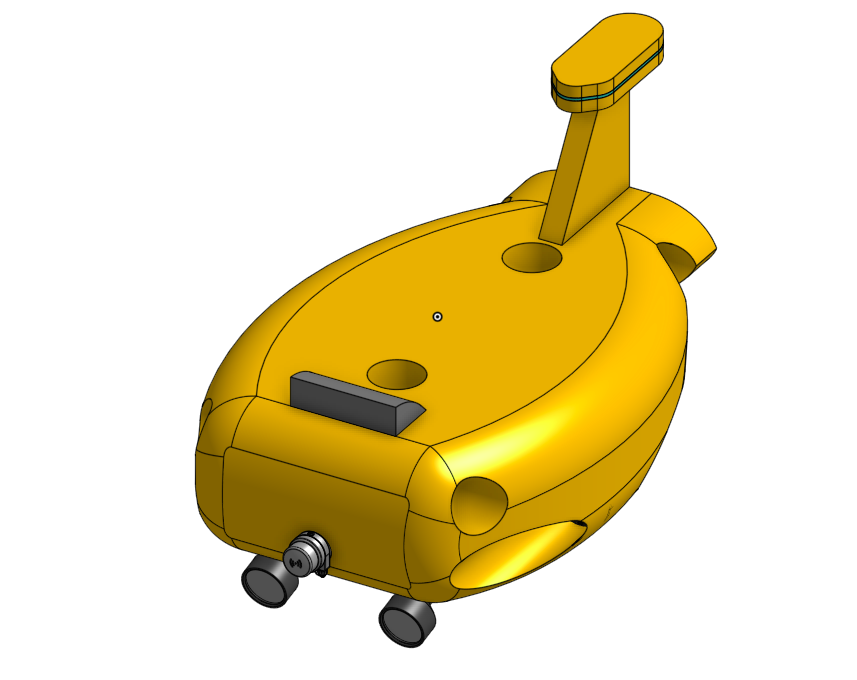
\includegraphics[width=.4\textwidth]{turbot-fish-01modi.png}
    \end{figure}
    
%*----------- notes
    \note[item]{Notes can help you to remember important information. Turn on the notes option.}
\end{frame}
%-
%*----------- SLIDE -------------------------------------------------------------
\begin{frame}[c]{Metodologia do projeto }
    %\transboxin[duration=1,direction=30]
        \begin{figure}
        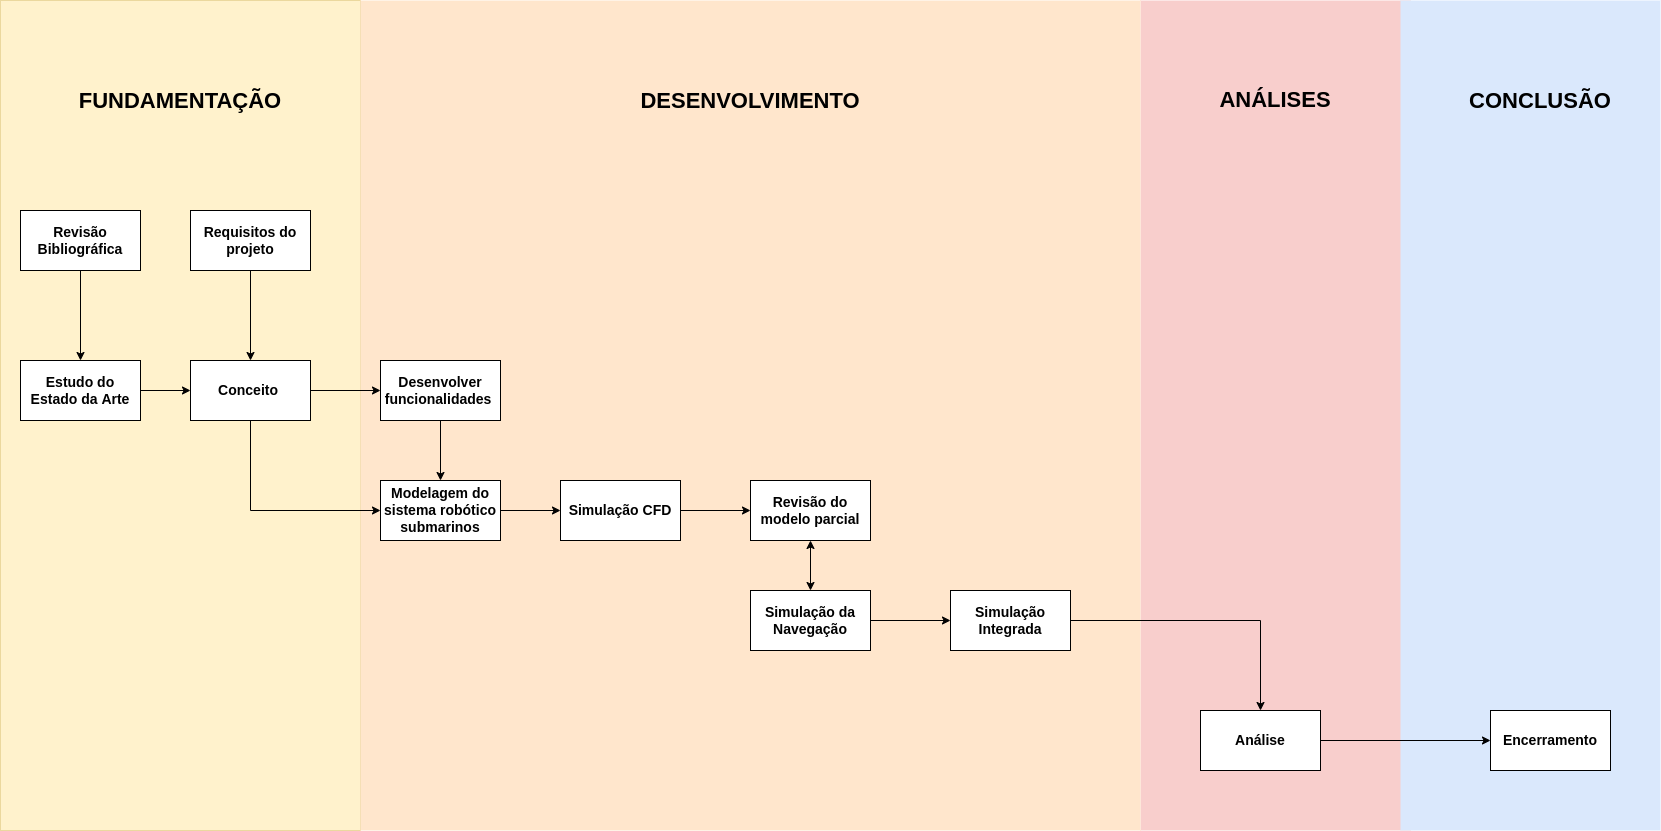
\includegraphics[width=.9\textwidth]{metodolodia2.png}
    \end{figure}
%*----------- notes
    \note[item]{Notes can help you to remember important information. Turn on the notes option.}
\end{frame}
%-
%*----------- SLIDE -------------------------------------------------------------
\begin{frame}[t]{Desenvolvido no projeto}
    \begin{itemize}
        \item Elaborado o cronograma do projeto
        \item Realizado o método BiLi
        \item Estudos sobre linguagens de programação C++, Python e R
        \item Estudo ROS e openFOAM
        \item Estudo sobre CFD (Fluidodinâmica computacional)
    \end{itemize}    
%*----------- notes
    \note[item]{Notes can help you to remember important information. Turn on the notes option.}
\end{frame}
%-
%*----------- SLIDE -------------------------------------------------------------
\begin{frame}[t]{Próximos passos do projeto}
    \begin{itemize}
        \item Listar as funcionalidades para desenvolvimento da montagem do sistema robótico submarino
        \item Simulação no OpenFOAM
        \item Simulação no ROS
        \item Desenvolvimento de 4 artigos: 
        \begin{itemize}
            \item[] 2022- SOTA e Simulação OpenFOAM
            \item[] 2023- DOE OpenFOAM e ROS 
        \end{itemize}   
        
    \end{itemize}    
%*----------- notes
    \note[item]{Notes can help you to remember important information. Turn on the notes option.}
\end{frame}
%-


